\documentclass[
a4paper,									% paper size
12pt,										% font size
oneside,									% one-page document
titlepage,									% there is a title page
parskip=half,								% distance between paragraphs (half line)
listof=totoc,								% list directories in the table of contents
bibliography=totoc,							% list bibliography in the table of contents
%footsepline,								% set foot line
]{scrreprt}



%\renewcommand{\familydefault}{\sfdefault}
\renewcommand*\familydefault{\rmdefault}		% family font
\usepackage[utf8]{inputenc}
\usepackage[T1]{fontenc}

\usepackage[margin=0.7in]{geometry}				% geometry settings in document
\usepackage[utf8]{inputenc}						% encoding
\usepackage{amsmath,amssymb,amsfonts,amsthm}	% related to math

\usepackage{multirow}  							% statement \multirow
\usepackage{graphicx}  							% statement \includegraphics
\usepackage{setspace}							% statement \begin{doublespace}
\usepackage{varioref}
%\usepackage[
%	automark,								 	% chapter in headline
%	headsepline,								% dividing line under header
%	ilines										% align the dividing line to the left
%]{scrpage2}

\usepackage[acronym,toc,automake]{glossaries}   % list of abbreviation, toc
\usepackage{scrlayer-scrpage}
\usepackage{color, xcolor}						% change the color of the font
\usepackage{calc}								% calculation

% show all cross-references and URLs as a link
\usepackage[
colorlinks=true, bookmarks, bookmarksnumbered, bookmarksopen, bookmarksopenlevel=1,
linkcolor=black, citecolor=black, urlcolor=blue, filecolor=blue,
pdfpagelayout=OneColumn, pdfnewwindow=true,
pdfstartview=XYZ, plainpages=false, pdfpagelabels,
pdfauthor={LyX Team}, pdftex,
pdftitle={LyX's Figure, Table, Floats, Notes, and Boxes manual},
pdfsubject={LyX-documentation about figures, tables, floats, notes, and boxes},
pdfkeywords={LyX, Tables, Figures, Floats, Boxes, Notes}]{hyperref}

\usepackage{textcomp,units}

\usepackage{booktabs}

\usepackage{listings}

\usepackage[german]{babel}


\usepackage{subfigure}
\usepackage[figure]{hypcap}

\usepackage{hyperref}

\definecolor{mygreen}{rgb}{0,0.6,0}
\definecolor{mygray}{rgb}{0.83,0.83,0.83}
\definecolor{mymauve}{rgb}{0.58,0,0.82}

\lstset{ 
  backgroundcolor=\color{mygray},   % choose the background color; you must add \usepackage{color} or 
  basicstyle=\footnotesize,        % the size of the fonts that are used for the code
  breakatwhitespace=false,         % sets if automatic breaks should only happen at whitespace
  breaklines=true,                 % sets automatic line breaking
  captionpos=b,                    % sets the caption-position to bottom
  commentstyle=\color{mygreen},    % comment style
  deletekeywords={...},            % if you want to delete keywords from the given language
  escapeinside={\%*}{*)},          % if you want to add LaTeX within your code
  extendedchars=true,              % lets you use non-ASCII characters; for 8-bits encodings only, does not work with UTF-8
  frame=single,	                   % adds a frame around the code
  keepspaces=true,                 % keeps spaces in text, useful for keeping indentation of code (possibly needs columns=flexible)
  keywordstyle=\color{blue},       % keyword style
  language=bash,                 % the language of the code
  morekeywords={sudo, cp, wget, apt-get, mkdir},            % if you want to add more keywords to the set
  numbers=left,                    % where to put the line-numbers; possible values are (none, left, right)
  numbersep=5pt,                   % how far the line-numbers are from the code
  numberstyle=\tiny\color{mygray}, % the style that is used for the line-numbers
  rulecolor=\color{black},         % if not set, the frame-color may be changed on line-breaks within not-black text (e.g. comments (green here))
  showspaces=false,                % show spaces everywhere adding particular underscores; it overrides 'showstringspaces'
  showstringspaces=false,          % underline spaces within strings only
  showtabs=false,                  % show tabs within strings adding particular underscores
  stepnumber=2,                    % the step between two line-numbers. If it's 1, each line will be numbered
  stringstyle=\color{mymauve},     % string literal style
  tabsize=2,	                   % sets default tabsize to 2 spaces
  title=\lstname                   % show the filename of files included with \lstinputlisting; also try caption instead of title
}						% load packages

% line spacing 1.5 lines
\onehalfspacing

% side edges
\setlength{\topskip}{\ht\strutbox} 
\geometry{paper=a4paper,left=30mm,right=30mm,top=10mm,bottom=40mm}



% head and foot line
%-------------------------------------------------------------
\pagestyle{scrheadings}
\renewcommand*{\chapterpagestyle}{scrheadings}

\renewcommand{\headfont}{\normalfont}			% font family of the header


% head line
%-------------------------------------------------------------
%\ihead{\small{\textsc{\titelum}}}  
\ihead{\textit{\headmark}}
%\ihead{\headmark}
\ohead{
\includegraphics[scale=0.12]{images/page_style/OTH_Regensburg_Logo_aktuell.jpg}}
\setlength{\headheight}{21mm} 					% height of the header

\setheadsepline[text]{0.4pt} 					% dividing line under header


% foot line
%-------------------------------------------------------------
%\setfootsepline[text]{0.4pt} 					% dividing line over foot
\cfoot{\textit{\pagemark}}
%\ofoot{}





% chapter number very large
\makeatletter
 \renewcommand*{\chapterformat}{ 
   \begingroup
     \setlength{\unitlength}{1mm}
     \begin{picture}(10,10)(0,5) 
       \setlength{\fboxsep}{0pt} 
       %\put(0,0){\framebox(20,40){}}% 
       %\put(0,20){\makebox(20,20){\rule{20\unitlength}{20\unitlength}}}% 
       \put(10,15){\line(1,0){\dimexpr 
           \textwidth-20\unitlength\relax\@gobble}}% 
       \put(0,0){\makebox(10,20)[r]{% 
           \fontsize{28\unitlength}{28\unitlength}\selectfont\thechapter 
           \kern-.05em
         }}
       \put(10,15){\makebox(\dimexpr 
           \textwidth-20\unitlength\relax\@gobble,\ht\strutbox\@gobble)[l]{ 
             \ \normalsize\color{black}\chapapp~\thechapter\autodot 
           }} 
     \end{picture} 
   \endgroup 
}
\makeatother

%set fonts for nicer pdf view
\IfFileExists{lmodern.sty}{\usepackage{lmodern}}
  {\usepackage[scaled=0.92]{helvet}
    \usepackage{mathptmx}
    \usepackage{courier} }
%\fi					% settings for page style


% A
\newacronym{ascii}{ASCII}{American Standard Code for Information Interchange}		% list of all abbreviations in document
\makeglossaries								% create glossary



\begin{document}							% begin document

% first inputs

\newgeometry{left=30mm,right=30mm,top=13mm,bottom=30mm} 

\titlepage

\begin{center}

\begin{tabular}{cc}
& \multirow{5}{*}{

\includegraphics[height=4.0cm]{images/cover_sheet/OTH_Regensburg_neues_Logo_01}}\tabularnewline

{\large{}Fakultät Informatik/Mathematik}\hspace{1.5cm} & \tabularnewline
 & \tabularnewline
 & \tabularnewline
 & \tabularnewline
\end{tabular}
\par\end{center}

\noindent 
\vspace{0.7cm}


\noindent \begin{center}
\textbf{\huge{}Projektstudium WS 18/19}
\par\end{center}{\Large \par}
\vspace{1.3cm}

\noindent
\rule{\textwidth}{0.3pt}
\vspace{0.1cm}

\begin{doublespace}
\noindent \begin{center}
{\Large{Verbesserter Aufbau eines \textbf{A}utonomen \textbf{L}aser \textbf{F}ahrzeugs (ALF)}}
\par\end{center}{\large \par}
\end{doublespace}
\noindent\rule{\textwidth}{0.3pt}



%\begin{center}
%\includegraphics[height=1.3cm]{images/cover_sheet/Bertrandt}
%\end{center}

\vspace{2.6cm}


%\begin{center}
\hskip 2.0cm
\begin{small}
%\renewcommand{\arraystretch}{1.2}
\begin{tabular}{ll}
eingereicht von:\hspace{0.7cm} & Bierschneider Christian, 3118760 \tabularnewline
 & Beck Dennis, \hspace{1.75cm} 3119329 \tabularnewline
 & Grauvogl Stefan, \hspace{1.15cm} 3119035 \tabularnewline
 & Studiengang: Informatik\tabularnewline
 & Schwerpunkt: Technische Informatik \tabularnewline
 & \tabularnewline
 
 
betreut durch: & Prof. Dr. Alexander Metzner\tabularnewline
 & OTH Regensburg\tabularnewline
 & \tabularnewline
  & \tabularnewline
\multicolumn{2}{l}{Regensburg, \today}\tabularnewline
\end{tabular}
\end{small}					% cover sheet

\pagenumbering{roman}						% i, ii, iii, iv
\restoregeometry							% restore geometry for document



\vspace{15.0mm}


\addchap{Abstract}


Here is space for a fancy short summary.						% abstract


% print list of abbreviation
\printglossary[
		type=\acronymtype,
		style=long,
		nonumberlist,
		title=List of Abbreviations
	]

%\renewcommand*\familydefault{\rmdefault}

% print table of contents
\tableofcontents{}

\newpage

\pagenumbering{arabic}						% change numbering to 1, 2, 3

\renewcommand*{\chapterpagestyle}{plain}    % redefine the chapter page style 

%insert all chapters here


\chapter{Introduction}


\section{Example for itemization }

Following an example for itemization and how it looks like
\begin{itemize}
\item item 1
\item item 2
\item item 3
\item item 4
\item item 5
\item item 6
\end{itemize}

\section{Section with abbrevations}

Just to show, what it looks like in the list of abbrevations

\acrfull{ascii}

\section{Further section}

Examples for a subsection

\subsection{Example for a subsection}



\subsubsection{Example for a subsubsection}






\chapter{Example with picture}

Here we test picture and how this is shown


\section{Picture with subtitle}

\begin{figure}[h]
\noindent \begin{centering}
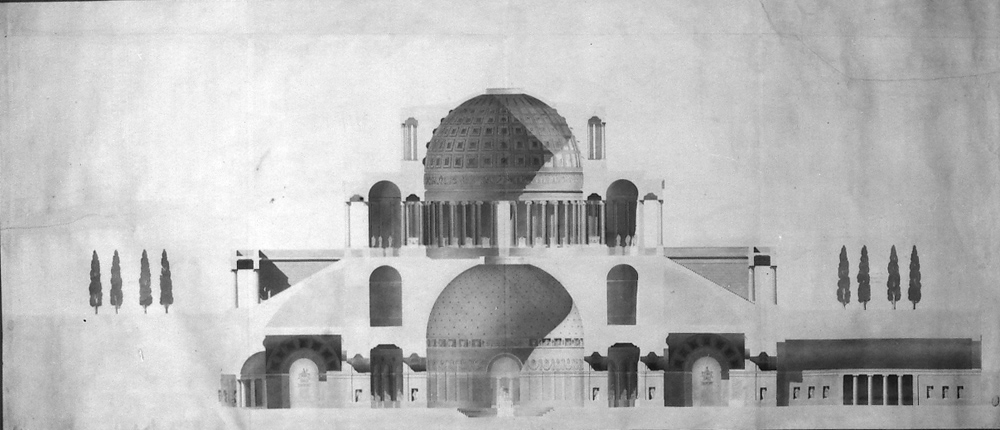
\includegraphics[width=15cm]{images/chapter2/1799_Diplomarbeit_Schnitt}
\par\end{centering}

\protect\caption[Short title which is only displayed in the list of figures]{This is a very long text. Here the picture should be described like this be that you also have an idea of the picture, if only the subtitle read \label{fig:testpicture}}
\end{figure}


In this text, i refer to the above-mentioned picture (see figure \vref{fig:testpicture}). For this, a so called brand has to be inserted in the picture ( in this case: fig:testpicture). As image width is in this document 15cm chosen. This looks very passable in the text out. Try to stay consistent with the widths of the pictures. So 15cm and 10cm for example. This helps the reader and does not interrupt constantly in the reading flow.

\newpage

\section{A section on a new page in the same chapter}
\chapter{Verwendetes Betriebssystem}
In diesem Kapitel wird die Installation des Betriebssystem Ubuntu Mate sowie die Einrichtung des Frameworks ROS näher erläutert. Außerdem werden alle nötigen Konfigurationen gezeigt, um die Software kompilieren und ausführen zu können. 


\section{Installation von Ubuntu Mate auf Raspberry Pi 3b+}
Aufgrund einer sehr großen Ubuntu Community und die gute Anbindung an das Framework ROS, wurde sich für das Betriebssystem Ubuntu Mate entschieden. Da keine durchgängige Echtzeitanbindung gefordert ist, werden hier der SLAM sowie die Wegfindung berechnet und ausgeführt. Die Sensoren der Motorsteuerung agieren dagegen auf dem STM32 Board (Abb. \ref{pic:STM32NucleoBoardPicture}) um schneller auf Änderungen reagieren zu können.\\ 
Da zum aktuellen Zeitpunkt (25.10.2018) kein angepasstes Betriebssystem für den Raspberry Pi 3b+ zur Verfügung steht, mussten kleinere Konfigurationen stattfinden um das vorhandene Raspberry Pi 3 Image auf einem Rasperry Pi 3b+ zum laufen zu bekommen. 
\textbf{Problem ohne diese Konfigurationen:} Der Raspberry Pi 3b+ startet nicht und es wird nur ein Regenbogen Bildschirm angezeigt!

Nachfolgend werden alle Konfigurationen erläutert, um ein neues Image zu flashen. 

1. Download eines Images für Raspberry  Pi 2/3 auf folgender Seite \href{https://ubuntu-mate.org/download/}{Ubuntu Mate}:

2. Flashen des Images auf eine SD-Karte mit Win32DiskImages (Windows) oder dd (linux):

3. Diese SD-Karte in einen \textbf{Raspberry Pi 2} oder \textbf{Raspberry Pi 3} einstecken und starten. 

4. Danach ein Terminal öffnen und folgenden Befehl für ein Kernel Update eingeben:\\

\begin{lstlisting}
$ sudo CURL_CA_BUNDLE=/etc/ssl/certs/ca-certificates.crt rpi-update
\end{lstlisting}
\vspace{-0.8cm}

oder alternativ:\\

\begin{lstlisting}
$ sudo BRANCH=stable rpi-update
\end{lstlisting}
\vspace{-0.8cm}

5. Raspberry Pi 2/3 herunterfahren und diese SD-Karte in den Raspberry Pi 3b+ einstecken. Der Pi sollte dann wie gewünscht booten. 

6. Zu diesem Zeitpunkt ist aber noch keine Wlan-Verbindung verfügbar. Installiere das neueste \href{https://www.raspberrypi.org/downloads/raspbian/}{Raspbian Image} auf eine weitere SD-Karte. 

7. Starte einen Raspberry Pi mit dem Raspbian Betriebssystem und kopiere folgenden Ordner (brcm (enthält wifi Treiber)) auf einen USB-Stick.\\

\begin{lstlisting}
$ sudo cp -r /lib/firmware/brcm /path_to_usb
\end{lstlisting}
\vspace{-0.8cm}

8. Starte den Raspberry Pi 3b+ mit der SD-Karte auf der Ubuntu Mate installiert ist. 

9. Ersetze den aktuellen /lib/firmware/brcm Ordner durch den am USB-Stick\\

\begin{lstlisting}
$ sudo cp -r /path_to_usb/lib/firmware/brcm /lib/firmware/brcm
\end{lstlisting}
\vspace{-0.8cm}

10. Führe einen Neustart durch und eine Wlan-Verbindung sollte verfügbar sein.

11. Aktiviere ssh durch folgenden Befehl\\

\begin{lstlisting}
$ sudo systemctl enable ssh
\end{lstlisting}


Aktueller Hostname und Passwort um per SSH auf den Raspberry Pi zugreifen zu können:\\
\textbf{Hostname: hsp}\\
\textbf{Passwort: hsp}







\section{Installation des Frameworks Robot Operating System (ROS)}

Nachfolgend wird Installation des Frameworks ROS durchgeführt. Dazu auf dem Betriebssystem Ubuntu Mate ein Terminal öffnen und folgende Befehle eingeben:

1. Einrichten der sources.list\\

\begin{lstlisting}
$ sudo sh -c 'echo "deb http://packages.ros.org/ros/ubuntu $(lsb_release -sc) main" > /etc/apt/sources.list.d/ros-latest.list'
\end{lstlisting}
\vspace{-0.8cm}

2. Einrichten der keys\\

\begin{lstlisting}
$ wget http://packages.ros.org/ros.key -O - | sudo apt-key add -
\end{lstlisting}
\vspace{-0.8cm}

3. Update der Packages\\

\begin{lstlisting}
$ sudo apt-get update
\end{lstlisting}
\vspace{-0.8cm}

4. Installation des ros-kinetic-desktop-full\\

\begin{lstlisting}
$ sudo apt-get install ros-kinetic-desktop-full
\end{lstlisting}
\vspace{-0.8cm}

5. Initialisierung und Update der Rosdep\\

\begin{lstlisting}
$ sudo rosdep init
\end{lstlisting}

\begin{lstlisting}
$ rosdep update
\end{lstlisting}
\vspace{-0.8cm}

6. Einrichten der ROS Umgebungsvariablen\\

\begin{lstlisting}
$ echo "source /opt/ros/kinetic/setup.bash" >> ~/.bashrc
\end{lstlisting}
\vspace{-0.8cm}

Neues Terminal öffnen oder nachfolgenden Befehl eingeben:\\

\begin{lstlisting}
$ source ~/.bashrc
\end{lstlisting}
\vspace{-0.8cm}

7. Erstellen eines catkin workspaces \\

\begin{lstlisting}
$ mkdir -p ~/catkin_ws/src
\end{lstlisting}

\begin{lstlisting}
$ cd ~/catkin_ws/
\end{lstlisting}

\begin{lstlisting}
$ catkin_make
\end{lstlisting}

\begin{lstlisting}
$ source ~/catkin_ws/devel/setup.bash
\end{lstlisting}
\vspace{-0.8cm}

Durch nachfolgenden Befehl hat man von überall im Linux System Zugriff auf die im catkin workspace gebildeten Packages:\\ 

\begin{lstlisting}
$ echo `source ~/catkin_ws/devel/setup.bash` << ~/.bashrc
\end{lstlisting}







\section{Schreibzugriff auf den Hokuyo Port für den aktuellen Benutzer}
Um nicht Root Rechte besitzen zu müssen um auf den Hokuyo Port zugreifen zu können, wurde der akuelle Benutzer (\textbf{hsp}) in die Dialout Gruppe mit folgendem Befehl hinzugefügt:\\

\begin{lstlisting}
$ sudo adduser hsp dialout
\end{lstlisting}

\vspace{-1.2cm}










\section{Roscore Master und Launch file als Systemd Service}
Da sich die SLAM Map sofort nach dem Start aufbauen soll, wurde sich für \textit{systemd services} entschieden. Diese werden beim hochfahren des Raspberry Pi 3b+ ausgeführt, außerdem kann der jeweilige Service auch nachträglich per Kommando gestartet und gestoppt werden.\\ 
Da der \textit{Roscore} Master benötigt wird, um innerhalb des ROS Frameworks zu kommunizieren, wurde dieser als einzelner Service entworfen. Hierfür muss unter \textit{/etc/systemd/system} eine Datei \textit{roscore.service} mit folgendem Inhalt erstellt werden.\\


\begin{lstlisting}
[Unit]
Description=starts roscore master as a systemd service

[Service]
Type=simple
ExecStart=/bin/bash -c "source /opt/ros/kinetic/setup.bash; /usr/bin/python /opt/ros/kinetic/bin/roscore"

[Install]
WantedBy=multi-user.target
\end{lstlisting}

\vspace{-0.9cm}
Um das ROS Launch File \textit{hokuyo\_hector\_slam.launch} als Service auszuführen, wurde eine Datei \textit{hector.service} in \textit{/etc/systemd/service} mit folgendem Inhalt erstellt.\\

\begin{lstlisting}
[Unit]
Description=starts hokuyo_hector_slam launch file as a systemd service

[Service]
Type=simple
ExecStart=/bin/bash -c "source /opt/ros/kinetic/setup.bash; source /path_to_catkin_ws/devel/setup.bash; /opt/ros/kinetic/bin/roslaunch /path/to/launch/file.launch"
Restart=on-failure

[Install]
WantedBy=multi-user.target
\end{lstlisting}

Wobei der Pfad zum \textit{catkin workspace} und der Pfad des Launch Files angegeben werden müssen.\\
Um diese Services beim hochfahren des Raspberry Pis zu starten, müssen diese erst mit nachfolgendem Befehl aktiviert werden.\\

\begin{lstlisting}
$ sudo systemctl enable roscore.service
$ sudo systemctl enable hector.service
\end{lstlisting}

Um den aktuellen Status dieser Services zu begutachten, muss folgender Befehl eingegeben werden. \textit{Status} kann auch durch \textit{restart} oder \textit{stop} ersetzt werden.\\ 

\begin{lstlisting}
$ sudo systemctl status roscore.service
$ sudo systemctl status hector.service
\end{lstlisting}
\vspace{-1.1cm}









\section{WiringPi Update}

Durch die Installation des Betriebssystems Ubuntu Mate kann es möglich sein, dass die Bibliothek \textbf{WiringPi} geupdated werden muss. Die Funktionsweise kann mit nachfolgendem Befehl überprüft werden, sollten Fehlermeldungen auftreten so muss die aktuelle Version durch die neueste Version ersetzt werden.\\

\begin{lstlisting}
$ gpio -v
\end{lstlisting}
\vspace{-0.8cm}

Sind Fehlermeldungen ersichtlich, muss die vorhandene Version ersetzt werden mit: \\

\begin{lstlisting}
$ sudo apt-get purge wiringpi
\end{lstlisting}
\vspace{-0.8cm}

Zuerst muss die aktuellste Version geklont und anschließend kompiliert werden.\\

\begin{lstlisting}
$ sudo apt-get install git
$ git clone git://git.drogon.net/wiringPi
$ cd wiringPi
$ ./build
\end{lstlisting}
\vspace{-0.8cm}

Zuletzt noch die Funktionsweise überprüfen:\\

\begin{lstlisting}
$ gpio -v 
$ gpio readall
\end{lstlisting}

\chapter{Verwendetes Betriebssystem}
In diesem Kapitel wird die Installation des Betriebssystem Ubuntu Mate, sowie die Einrichtung des Frameworks ROS näher erläutert. Außerdem werden alle nötigen Konfigurationen gezeigt, um die Software kompilieren und ausführen zu können. 


\section{Installation von Ubuntu Mate auf Raspberry Pi 3b+}
Aufgrund einer sehr großen Ubuntu Community und die gute Anbindung an das Framework ROS, wurde sich für das Betriebssystem Ubuntu Mate entschieden. Da keine durchgängige Echtzeitanbindung gefordert ist, werden hier der SLAM sowie die Wegefindung berechnet und ausgeführt. Die Sensoren der Motorsteuerung agieren dagegen auf einem STM Board um schneller auf Änderungen reagieren zu können. 
Da zum aktuellen Zeitpunkt (25.10.2018) kein angepasstes Betriebssystem für den Raspberry Pi 3b+ zur Verfügung steht, mussten kleinere Konfigurationen stattfinden um das vorhandene Raspberry Pi 3 Image auf einem Rasperry Pi 3b+ zum laufen zu bekommen. 
Problem ohne diese Konfigurationen: Der Raspberry Pi 3b+ startet nicht und es wird nur ein Regenbogen Bildschirm angezeigt!

Nachfolgend werden alle Konfigurationen erläutert, um ein neues Image zu flashen. 

1. Download eines Images für Raspberry  Pi 2/3 auf folgender Seite \href{https://ubuntu-mate.org/download/}{Ubuntu Mate}:

2. Flashen des Images auf eine SD-Karte mit Win32DiskImages (Windows) oder dd (linux):

3. Diese SD-Karte in einen \textbf{Raspberry Pi 2} oder \textbf{Raspberry Pi 3} einstecken und starten. 

4. Danach ein Terminal öffnen und folgenden Befehl für ein Kernel Update eingeben:\\

\begin{lstlisting}
$ sudo CURL_CA_BUNDLE=/etc/ssl/certs/ca-certificates.crt rpi-update
\end{lstlisting}

oder alternativ:\\

\begin{lstlisting}
$ sudo BRANCH=stable rpi-update
\end{lstlisting}

5. Raspberry Pi 2/3 herunterfahren und diese SD-Karte in den Raspberry Pi 3b+ einstecken. Der Pi sollte dann wie gewünscht booten. 

6. Zu diesem Zeitpunkt ist aber noch keine Wlan-Verbindung verfügbar. Installiere das neueste Raspbian Image von hier auf eine weitere SD-Karte. 

7. Starte einen Raspberry Pi mit dem Raspbian Betriebssystem und kopiere folgenden Ordner auf einen USB-Stick.\\

\begin{lstlisting}
$ sudo cp -r /lib/firmware/brcm /path_to_usb
\end{lstlisting}

8. Starte den Raspberry Pi 3b+ mit der SD-Karte auf der Ubuntu Mate installiert ist. 

9. Ersetze den aktuellen /lib/firmware/brcm Ordner durch den am USB-Stick\\

\begin{lstlisting}
$ sudo cp -r /path_to_usb/lib/firmware/brcm /lib/firmware/brcm
\end{lstlisting}

10. Führe einen Neustart durch und eine Wlan-Verbindung sollte verfügbar sein.

11. Aktiviere ssh durch folgenden Befehl\\

\begin{lstlisting}
$ sudo systemctl enable ssh
\end{lstlisting}


Aktueller Hostname und Passwort um per SSH auf den Raspberry Pi zugreifen zu können:\\
\textbf{Hostname: hsp}\\
\textbf{Passwort: hsp}

\section{Installation des Frameworks Robot Operating System (ROS)}

Nachfolgend wird Installation des Frameworks ROS durchgeführt. Dazu auf dem Betriebssystem Ubuntu Mate ein Terminal öffnen und folgende Befehle eingeben:

1. Einrichten der sources.list\\

\begin{lstlisting}
$ sudo sh -c 'echo "deb http://packages.ros.org/ros/ubuntu $(lsb_release -sc) main" > /etc/apt/sources.list.d/ros-latest.list'
\end{lstlisting}

2. Einrichten der keys\\

\begin{lstlisting}
$ wget http://packages.ros.org/ros.key -O - | sudo apt-key add -
\end{lstlisting}

3. Update der Packages\\

\begin{lstlisting}
$ sudo apt-get update
\end{lstlisting}

4. Installation des ros-kinetic-desktop-full\\

\begin{lstlisting}
$ sudo apt-get install ros-kinetic-desktop-full
\end{lstlisting}

5. Initialisierung und Update der Rosdep\\

\begin{lstlisting}
$ sudo rosdep init
\end{lstlisting}

\begin{lstlisting}
$ rosdep update
\end{lstlisting}

6. Einrichten der ROS Umgebungsvariablen\\

\begin{lstlisting}
$ echo "source /opt/ros/kinetic/setup.bash" >> ~/.bashrc
\end{lstlisting}

Neues Terminal öffnen oder nachfolgenden Befehl eingeben:\\

\begin{lstlisting}
$ source ~/.bashrc
\end{lstlisting}

7. Erstellen eines catkin workspaces \\

\begin{lstlisting}
$ mkdir -p ~/catkin_ws/src
\end{lstlisting}

\begin{lstlisting}
$ cd ~/catkin_ws/
\end{lstlisting}

\begin{lstlisting}
$ catkin_make
\end{lstlisting}

\begin{lstlisting}
$ source ~/catkin_ws/devel/setup.bash
\end{lstlisting}

Durch nachfolgenden Befehl hat man von überall im Linux System Zugriff auf die im catkin workspace gebildeten Packages:\\ 

\begin{lstlisting}
$ echo `source ~/catkin_ws/devel/setup.bash` << ~/.bashrc
\end{lstlisting}

\section{Schreibzugriff auf den Hokuyo Port für den aktuellen Benutzer}
Um nicht Root Rechte besitzen zu müssen um auf den Hokuyo Port zugreifen zu können, wurde der akuelle Benutzer in die Dialout Gruppe mit folgendem Befehl hinzugefügt:\\

\begin{lstlisting}
$ sudo adduser "user_name" dialout
\end{lstlisting}

\section{Roscore Master und Launch file als Systemd Service}
Da sich die SLAM Map sofort nach dem Start aufbauen soll, wurde sich für systemd services entschieden. Diese werden beim hochfahren des Raspberry Pi 3b+ ausgeführt, außerdem kann der jeweilige Service auch nachträglich per Kommando gestartet und gestoppt werden. 
Da der roscore Master benötigt wird, um innerhalb des ROS Frameworks zu kommunizieren, wurde dieser als einzelner Service entworfen. Hierfür muss unter /etc/systemd/system eine Datei roscore.service mit folgendem Inhalt erstellt werden.\\


\begin{lstlisting}
[Unit]
Description=starts roscore master as a systemd service

[Service]
Type=simple
ExecStart=/bin/bash -c "source /opt/ros/kinetic/setup.bash; /usr/bin/python /opt/ros/kinetic/bin/roscore"

[Install]
WantedBy=multi-user.target
\end{lstlisting}

Um das ROS launch File hokuyo\_hector\_slam.launch als Service auszuführen wurde eine Datei hector.service in /etc/systemd/service mit folgendem Inhalt erstellt.\\

\begin{lstlisting}
[Unit]
Description=starts hokuyo_hector_slam launch file as a systemd service

[Service]
Type=simple
ExecStart=/bin/bash -c "source /opt/ros/kinetic/setup.bash; /usr/bin/python /opt/ros/kinetic/bin/roscore"
ExecStop=
Restart=on-failure

[Install]
WantedBy=multi-user.target
\end{lstlisting}


\chapter{Hardware}

\section{Lidar}

Als Laserscanner wird ein Hokuyo URG-04LX verwendet.

Dieser hat eine Auflösung von 360° / 1024 pro Step. Insgesamt kann ein Winkel von 240° (= 768 Datenpunkte) je Scan aufgezeichnet werden.

\begin{figure}[h]
\begin{center}
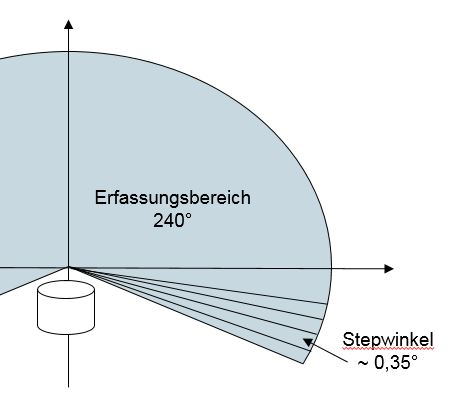
\includegraphics[width=10cm]{images/chapter5/LidarHardware.jpg}
\caption{Lidar Uebersicht}
\label{Lidar_uebersicht}
\end{center}
\end{figure}

Die Daten werden für jeden erfassten Punkt jeweils im Abstand von 0,35° als Entfernung geliefert. Die Punkte sind somit in Polarkoordinaten Darstellung vorhanden.

\begin{figure}[h]
\begin{center}
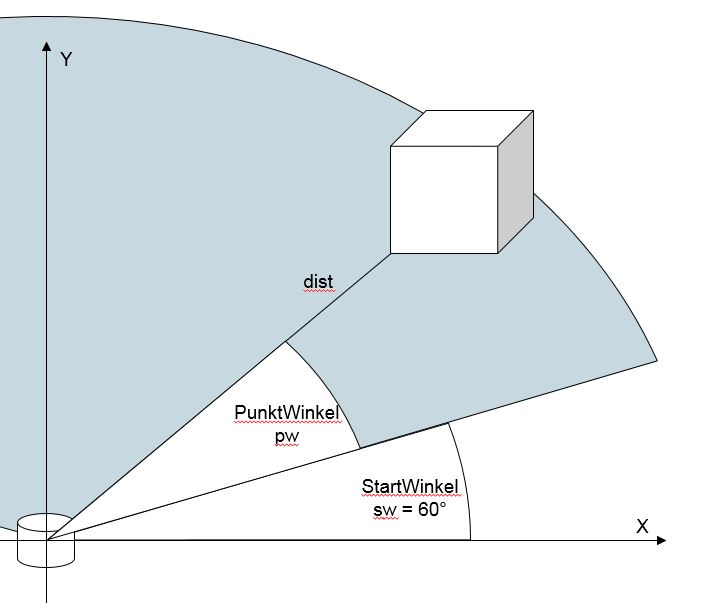
\includegraphics[width=10cm]{images/chapter5/LidarWinkeluebersicht.jpg}
\caption{Lidar Uebersicht}
\label{Lidar_uebersicht}
\end{center}
\end{figure}





\chapter{Software}



Nachfolgend wird das Design dieses Softwareprojekts dargestellt, sowie die leichte Erweiterung durch nachträgliche Module. Anschließend wird noch auf die bereits umgesetzten Module eingegangen und ihre Funktionsweise erklärt. 


\section{Design des Projektes mit CMake}

\section{Verbindung zum Lidar}

Der Lidar Sensor ist direkt via USB mit dem Raspberry Pi verbunden. Die Daten werden vom Lidar in Polarkoordinaten Darstellung geliefert. Um eine Karte aufbauen zu können, wurde ein Modul erstellt, das die Daten in kartesische Koordinaten transformiert. Somit ist es möglich nach jeder Messung des Lidars eine neue Karte mit der \"aktuellen Sicht\" des Sensors zu erstellen. Die Daten werden in einem Integer-Array gespeichert und können von einem SLAM Algorithmus verarbeitet werden . 

Das Modul verwendet zur Verbindung mit dem Lidar die unter der GNU GPL v3 stehende API \"URG04LX\". Mit ihr ist es möglich einen kompletten Scan des Lidars aufzuzeichnen. 

\begin{lstlisting}
int data[MEASUREMENT_POINTS]; 
int measuredPoints;
URG04LX laser;

laser = URG04LX('dev/tty/ACM0')

measuredPoints = laser.getScan(data);

\end{lstlisting}

Die Datenpunkte werden in polarkoordinaten Darstellung geliefert und müssen zur Weiterverarbeitung in kartesische Koordinaten umgerechnet werden. 

\begin{figure}[h]
\begin{center}
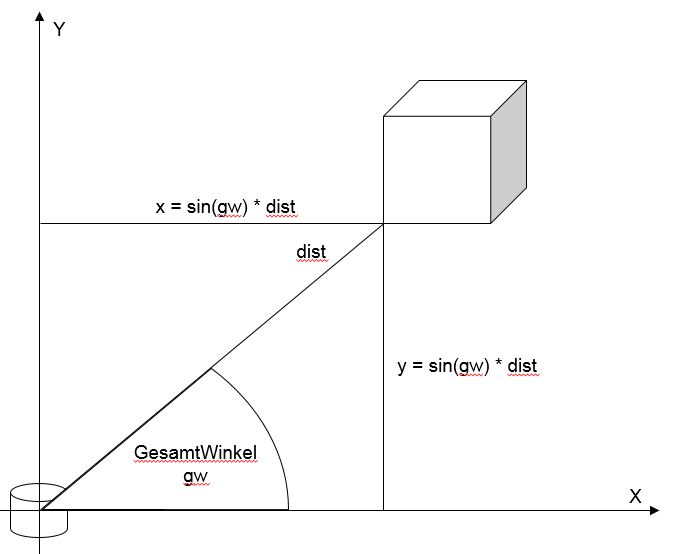
\includegraphics[width=10cm]{images/chapter5/LidarKoordRechnung.jpg}
\caption{Koordinaten errechnen}
\label{Koordinaten_errechnen}
\end{center}
\end{figure}

Die Umrechnung muss für alle aufgezeichneten Datenpunkte des Scans vorgenommen werden und liefert dann die Sicht des Lidars in einem Koordinatensystem:

\begin{figure}[h]
\begin{center}
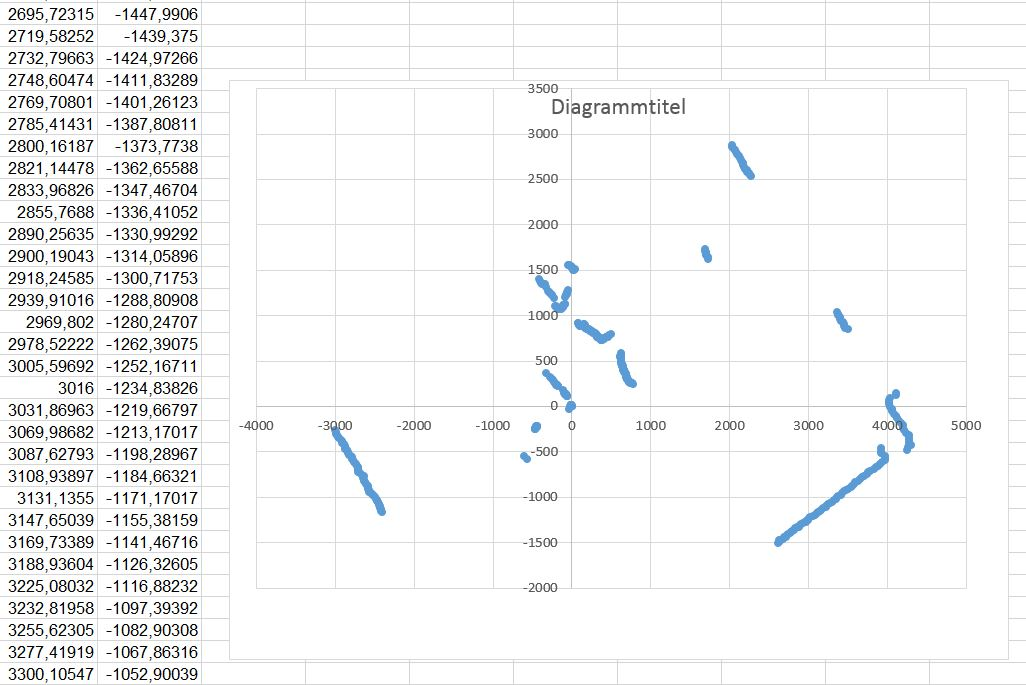
\includegraphics[width=10cm]{images/chapter5/kartKoord.jpg}
\caption{Koordinaten Veranschaulichung}
\label{Koordinaten_veranschaulichung}
\end{center}
\end{figure}




Das Modul wird momentan nicht verwendet, da der SLAM Algorithmus mit Hilfe von ROS realisiert wurde und die entsprechende Library einen eigenen Connector zum Lidar bereitstellt. Um folgenden Gruppen jedoch die Arbeit zu erleichtern, wurde das Modul trotzdem vorbereitet.



\section{SLAM}

\section{Wegefindung}


Vorüberlegung:
Das definierte Ziel ALF autonom einen Raum erkunden zu lassen, beinhaltet neben dem Erstellen einer Karte auch eine Wegberechnung zu unbekannten Flächen im Raum, die noch nicht vom Lidar erfasst wurden. Somit muss basierend auf der vom SLAM erstellten Karte ein Pfad zu den unbekannten Flächen gefunden werden.
Dabei muss berücksichtigt werden, dass ALF durch seine Lenkung einen eingeschränkten Aktionsradius hat und es nicht möglich ist aus einer Geradeaus-Fahrt sofort nach Rechts oder links abzubiegen. somit ist es nicht möglich direkt an einer Wand entlang "ums Eck" zu fahren. Der Lenkwinkel muss in die Routenplanung mit einbezogen werden. 

Eingabe: 
Karte als Matrix
Egoposition auf Karte


1) Übergabe Daten von SLAM

Die vom SLAM erhaltenen Daten entsprechen der einer PGM-Datei. In einem 2-dimensionalen Integer-Array wird die erstellte Karte als Grauwerte übergeben. Mögliche Werte sind 
erkanntes Objekt (Schwarz),  Unbekannte Fläche (Grau),  Freifläche(Weiß).


Beispiel: 
\begin{lstlisting}
[ 127 127 127 127 127 127 127 ... ]
[ 127 127 127 127 127 127 127 ... ]
[ 127  0   0   0   0  127 127 ... ]
[ 127  0  255 255 255 127 127 ... ]
[ 127  0  255 255 255 127 127 ... ]
[ 127  0  255 255 255 127 127 ... ]
[ 127  0  255 255 255 127 127 ... ]

0 = erkanntes Objekt
127 = unbekannte Flaeche
255 = Freiflaeche

\end{lstlisting}

2) Whiten

Die vom SLAM erhaltene Karte kann unter Umständen nicht nur Schwarze, Weiße und fest definierten graue Punkte enthalten. Je nach verwendetem SLAM werden für Messpunkte, die nicht sicher als Objekt oder Freifläche definiert werden können, als Zwischengrauwert angegeben. Dies führt jedoch bei der weiteren Berechnung des Pfades zu Problemen. Daher wurde eine Grenze definiert, unter der alle Punkte als Objekt und über der alle als Freifläche angesehen werden. Somit kann im weiteren Programm von sauberen Werten (Objekt, Freifläche, Unbekannt) ausgegangen werden. 

< Bild vor/nach whiten >


3) Gradientenfüllung

Zur Realisierung der in der Einleitung genannten Lenkwinkel-Problematik, wurde die Karte mit selbst definierten Grauwerten eingefärbt. Je weiter das Fahrzeug von einem Gegenstand bzw. einer Wand entfernt ist, desto unkritischer wird die Navigation mit dem Lenkwinkel. 
Freiflächen der Karte, die nahe an einer Wand liegen, sollen nach Möglichkeit gemieden werden. Punkte, die in der Mitte eines Raumes ohne Gegenstände liegen, werden als positiv für die Routenplanung angesehen. 
Somit sollte der Pfad immer zuerst in die Mitte eines Raumes führen und sich erst am Zielpunkt wieder einer Wand nähern. 
Umgesetzt wurde dies mit einer Grau-Gradientenfüllung der Karte, die später bei der Pfadberechnung als Gewichtung dienen. Die Freiflächenpunkte nahe einer Wand wurden mit einem hohen Gewicht (repräsentiert durch "dunkelgrau") belegt und verringern ihr Gewicht, je weiter sie von einer Wand entfernt liegen. 

<Bild graymapped>


4) in Graphen wandeln

Um auf der bestehenden Karte einen Pfad berechnen zu können, muss die Matrix in einen Graphen überführt werden. Die einfachste (wenn auch nicht die performanteste) Methode war es jeden Freiflächen-Messpunkt des Lidars als eigenen Knoten anzusehen, der eine Verbindung zu den jeweilig benachbarten Messpunkten/Knoten hat. Als Kantengewicht wurde der entsprechende Grauwert des Nachbarknoten gewählt. Somit werden Pfade auf Freiflächen belohnt (Kantengewicht = 0) und Annäherungen an Gegenstände bestraft (Kantengewicht = steigender Grauwert). 
Für unbekannte Flächen sowie erkannte Objekte wurden keine Knoten in den Graphen eingefügt und diese auch nicht als Nachbarn angesehen. 


\begin{figure}[h]
\begin{center}
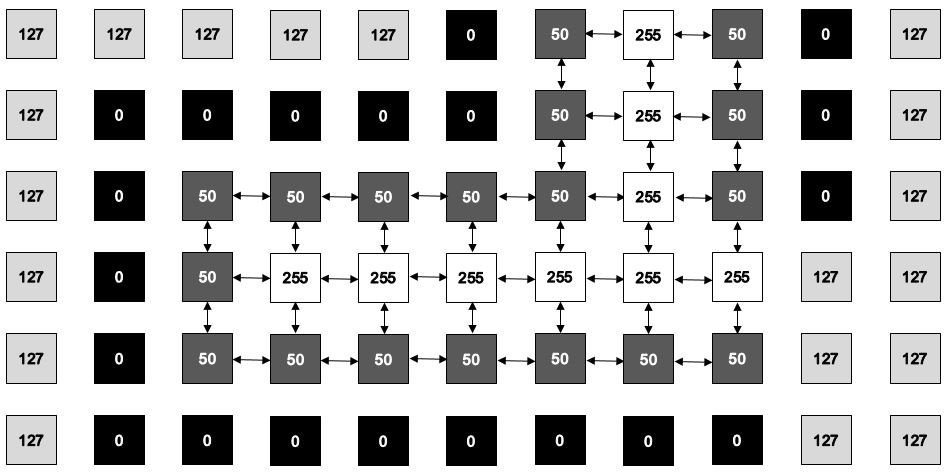
\includegraphics[width=15cm]{images/chapter5/GraphKnoten.jpg}
\caption{aus Map erstellter Graph}
\label{Map_aus_Graph}
\end{center}
\end{figure}


Dass aus jedem Pixel ein eigener Knoten wird, hat zur Folge, dass es extrem viele mögliche Pfade zu berechnen gibt. Hier existiert noch ein mögliches Verbesserungspotential für weitere Gruppenarbeiten. Da es sich jedoch um einen ersten autonomen Prototypen handelt, reicht die Umsetzung auf diesem Wege aus.




5) mögliche Ziele definieren und finden

Als Voraussetzung wird immer angenommen, dass die aktuelle Position des Fahrzeugs auf einer erkannten Freifläche liegt. Das übergeordnete Ziel einen Raum vollständig autonom zu erkunden, lässt sich nur erreichen, indem das Fahrzeug nicht zufällig durch den Raum fährt, sondern gezielt unbekannte Flächen ansteuert. Mögliche Ziele sind somit alle Übergänge von Freifläche zu unbekannter Fläche. 

Probleme:
Es kann passieren, dass der Lidar Sensor durch Reflektionen spiegelnder Oberflächen fehlerhafte Werte liefert. Somit entsteht bei der Verarbeitung der Daten mit dem SLAM der Eindruck, dass eine Freifläche hinter einer Wand erkannt wurde. Da es auch dort zu Übergängen zwischen Freifläche und Unbekanntem Bereich kommen kann, werden diese Punkte auch als mögliche, zu erkundende Ziele erkannt. Da es jedoch keinen Weg zu diesen separierten Freiflächen gibt, ist es nicht möglich einen Pfad zu berechnen. Da sich dies als großes, nur sehr schwierig zu lösendes Problem herausstellte, wurde als Workaround die Pfadsuche so implementiert, dass alle Ziele durchgetestet werden und die Pfadberechnung nur abgeschlossen ist, wenn ein gültiger Pfad gefunden werden konnte.

<Evtl Bild von allen unbekannten Übergängen>


6) Dijkstra

Der erstellte Graph kann nun mit Hilfe eines Dijkstra-Algorithmus den kürzesten Weg von der Egoposition zum einem der möglichen, erkannten Ziele errechnen. Die in 3) eingeführte Gewichtung der Kanten führt nun dazu, dass ein Weg z.B. in der Mitte eines Ganges entlang errechnet wird. Bei 90° Winkeln wird eine leichte Biegung errechnet. Die Kantengewichtung ist auf dem kürzeren Pfad zwar schlechter, jedoch ist der Weg kürzer. Somit wird auch die Lenkwinkelproblematik entschärft. 

Als Dijkstra-Implementierung wurde die Veröffentlichung von Mahmut Bulut als Grundlage verwendet und für das Projekt angepasst.

// https://gist.github.com/vertexclique/7410577


7) ersteller Pfad

Als Ergebnis des Dijkstra-Algorithmus wird ein Pfad von der Egoposition über die Freiflächen bis hin zu einer zufälligen, unbekannten Fläche erzeugt. Die Navigation des Fahrzeuges übernimmt das Bewegungssteuerungsmodul. Sobald das Ziel erreicht wurde, kann ein neuer Pfad zu den noch verbleibenden, unbekannten Flächen erzeugt werden.



allgemeine Laufzeitoptimierung -> Blocks

Der verwendete SLAM liefert eine Auflösung von XXXX m / Pixel. Zur Berechnung eines Pfades ist diese Auflösung jedoch zu detailiert, sodass die gesamte Karte in Blocks mit Freiflächen eingeteilt werden kann. Um die Laufzeit des Dijkstra zu verringern, wurde nicht jeder Pixel als Knoten angesehen, sondern ein Block von z.B. 5x5 Pixeln als 1 Knoten. Dies verringert zwar die Genauigkeit des Pfades, durch die Lenkwinkelproblematik wird diese jedoch sowieso nicht benötigt.



Ausgabe:
Pfad von Egoposition zu Freifläche





\section{Bewegungssteuerung}



Here i quote from a particular book: This quote is from one special book that i have to specify in the end. There are even two books, just so you see that \cite{Williams201205,Siegert200612}


Legislative texts, for example, need not to be quoted. Here is enough a reference in the footnote \footnote{This is the super footnote, here is something of BGB §§12 Abs. 3 Satz 4}


\renewcommand*{\chapterpagestyle}{scrheadings} % redefine the chapter page style 

% list of figures and add to toc
\listoffigures


% list of tables and add to toc
\listoftables


% attachment

~
\vspace{15.0mm}


\addchap{Anhang}



% bibliography
\bibliographystyle{bibtex/unsrtdin}
%\bibliographystyle{natdin}
\bibliography{bibtex/thesis}



\end{document}